\chapter{Methodology}
In this section, we will delve into the implementation aspect of the project. Initially, we will provide insights into the development of the Vake Map. Following that, we will elaborate on our modifications to integrate the RESCO repository into our specific use case. Subsequently, we will proceed to examine the system's evaluation, emphasizing its utilization of RESCO once more.

\section{Why Vake Street} \label{sec:why-vake}
In the pursuit of optimizing urban traffic flow, it is essential to begin by selecting a target street that encapsulates the complexity and challenges of urban traffic management. In this section, we delve into the rationale behind our choice of Vake Street as the focal point of our thesis.

\subsection{Significance of Vake Street}
First and foremost, Vake Street stands out as one of the most bustling thoroughfares in Tbilisi, the capital of Georgia. The significance of this street arises from multiple factors that converge to create a traffic scenario of paramount interest for our study.

\subsubsection{Academic Hub}
Vake Street is home to no fewer than eight universities, making it an academic hub of considerable proportions. The presence of numerous educational institutions along this stretch of road naturally attracts a substantial volume of students, faculty, and staff. This academic concentration contributes significantly to the street's vibrant and dynamic atmosphere.

\subsubsection{Business Epicenter}
Beyond its academic allure, Vake Street also boasts a reputation as a prime location for business enterprises. It hosts a multitude of offices, firms, and establishments, making it one of the preeminent commercial centers in Tbilisi. The clustering of business activities results in a constant influx of commuters and visitors, further intensifying the street's traffic dynamics.

\subsubsection{Residential Nexus}
In addition to its academic and commercial prominence, Vake Street encompasses a sizable residential area. The coexistence of educational institutions, businesses, and residential zones within the same vicinity engenders a unique traffic ecosystem. The daily routines of residents, including commuting and daily errands, contribute significantly to the overall traffic load.

\subsection{Traffic Challenges}
The confluence of these factors underscores the challenges presented by Vake Street's traffic management. The street's infrastructure consists mainly of narrow lanes, typically featuring only one or two lanes on each side, alongside a dedicated bus lane. Notably, the introduction of bus lanes in recent times has added an extra layer of complexity to the traffic dynamics.

\begin{figure}[h]
    \centering
    \begin{subfigure}{0.45\textwidth}
        \centering
        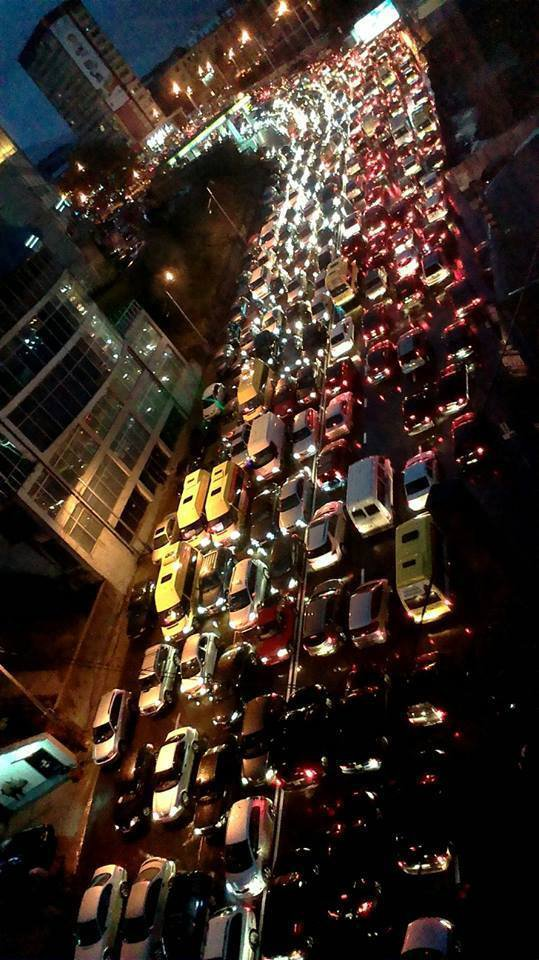
\includegraphics[width=\linewidth]{images/methodology/vake-traffic-1.jpg}
    \end{subfigure}
    \hfill
    \begin{subfigure}{0.45\textwidth}
        \centering
        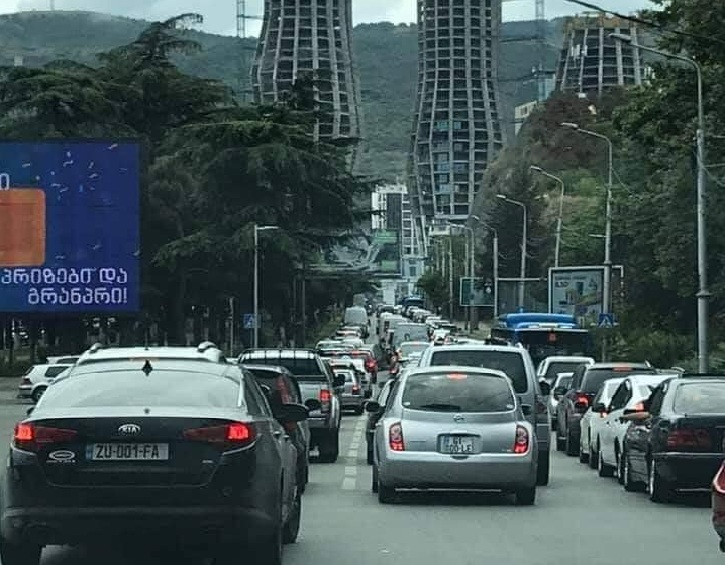
\includegraphics[width=\linewidth]{images/methodology/vake-traffic-2.jpg}
    \end{subfigure}
    \caption{Typical Traffic Scene on Vake Street}
    \label{fig:vake-real-traffic}
\end{figure}

Figure \ref{fig:vake-real-traffic} provides a visual glimpse into the daily traffic scenario on Vake Street. It showcases the challenges posed by congestion, narrow roadways, and the constant interplay between vehicles, pedestrians, and public transportation.

\subsection{Personal Connection}
To add a personal dimension to our choice of Vake Street, it is worth mentioning that I, too, have had a direct experience with this street. As a former student of one of the universities located on Vake Street, I have personally witnessed the intricacies and frustrations of navigating this busy thoroughfare. My firsthand encounters with the traffic issues on Vake Street further fueled my determination to tackle this complex urban traffic optimization problem.

In summary, Vake Street's confluence of academic institutions, business enterprises, and residential communities, coupled with its traffic challenges and my personal connection, make it an ideal candidate for our thesis on optimizing urban traffic flow.

\section{Creation of Vake Map} \label{sec:map-creation}

Before embarking on the simulation of urban traffic flow, it is imperative to have a map that closely mirrors the real-world environment. This level of realism is crucial for the accuracy and effectiveness of the simulation. In this section, we detail the process of creating the Vake map, which serves as the foundation for our traffic simulation.

\subsection{Utilizing Netedit}
To initiate the map creation process, we leveraged the powerful tool known as Netedit (Section \ref{sec:netedit}). This tool is instrumental in designing road networks for traffic simulations. However, the challenge we encountered was the need for an exceptionally precise representation of the map. Manual creation proved to be a laborious and time-consuming endeavor.

\subsection{Discovery of OpenStreetMap}
Fortunately, our quest for an accurate map led us to the discovery of an invaluable resource - the \href{http://openstreetmap.org}{OpenStreetMap (OSM)} platform. OpenStreetMap provides comprehensive and authentic maps, including detailed information about various regions, including the prominent streets of Vake in Georgia.

\begin{figure}[h]
    \centering
    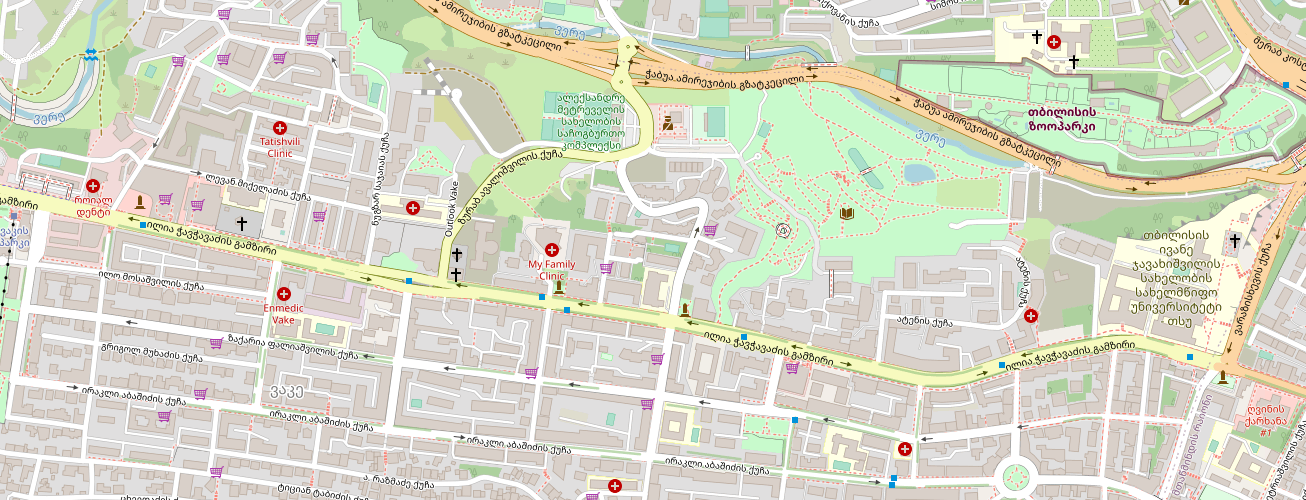
\includegraphics[width=1\linewidth]{images/methodology/vake-openstreetmap.png}
    \caption{Vake Map from OpenStreetMap}
    \label{fig:vake-openstreetmap}
\end{figure}

As depicted in Figure \ref{fig:vake-openstreetmap}, OpenStreetMap offers a user-friendly interface that allows us to select specific areas and generate map files with the extension \textbf{$.osm$}.

\subsection{Conversion with $netconvert$}
Once we obtained the OSM file, the next crucial step was the conversion of the map into a format compatible with the SUMO simulation environment. This conversion is accomplished using the SUMO tool called $netconvert$. 

However, it's worth noting that the process doesn't conclude here. OpenStreetMap provides a comprehensive map that includes numerous objects and details that are not relevant for our SUMO simulation. Moreover, $netconvert$ may introduce errors during the conversion process.

\newpage
\subsection{Refinement and Corrections}
To ensure the accuracy and relevance of our map for traffic simulations, we embarked on a meticulous process of refinement and correction. This involved the removal of extraneous objects from the map and the addition of specific details required for our simulation, such as bus lines that were not initially present in the OpenStreetMap data.

The effort invested in this refinement phase exceeded our initial expectations, primarily due to the need for extensive object removal and the inclusion of additional details.

\begin{figure}[h]
    \centering
    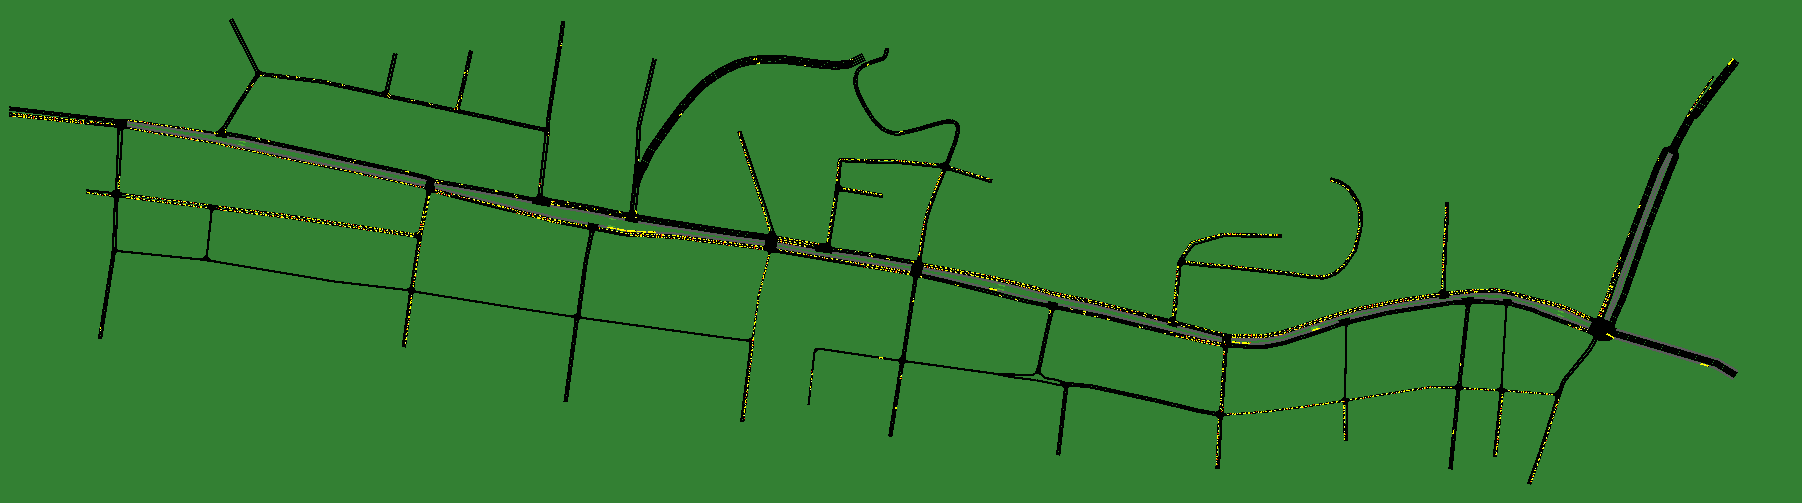
\includegraphics[width=1\linewidth]{images/methodology/vake-sumo.png}
    \caption{Vake Map for SUMO Simulation}
    \label{fig:vake-sumo}
\end{figure}

As seen in Figure \ref{fig:vake-sumo}, the result of our painstaking efforts is a map that faithfully replicates the shape and characteristics of the Vake area. This refined map serves as the groundwork for our subsequent traffic light control optimization experiments.

\section{Traffic Lights} \label{sec:tl}
Traffic lights play a pivotal role in regulating and controlling traffic flow on urban streets. In this section, we will delve into the intricate world of traffic lights, which serve as both the cause and the tool for managing traffic in the complex environment of Vake Street. We will provide an in-depth examination of each of the six traffic lights situated along this thoroughfare.

\subsection{Traffic Light 1} \label{sec:tl-1}
To commence our exploration of traffic lights, let's begin with an overview of Traffic Light 1, as depicted below:

\begin{figure}[h]
    \centering
    \begin{subfigure}{0.45\textwidth}
        \centering
        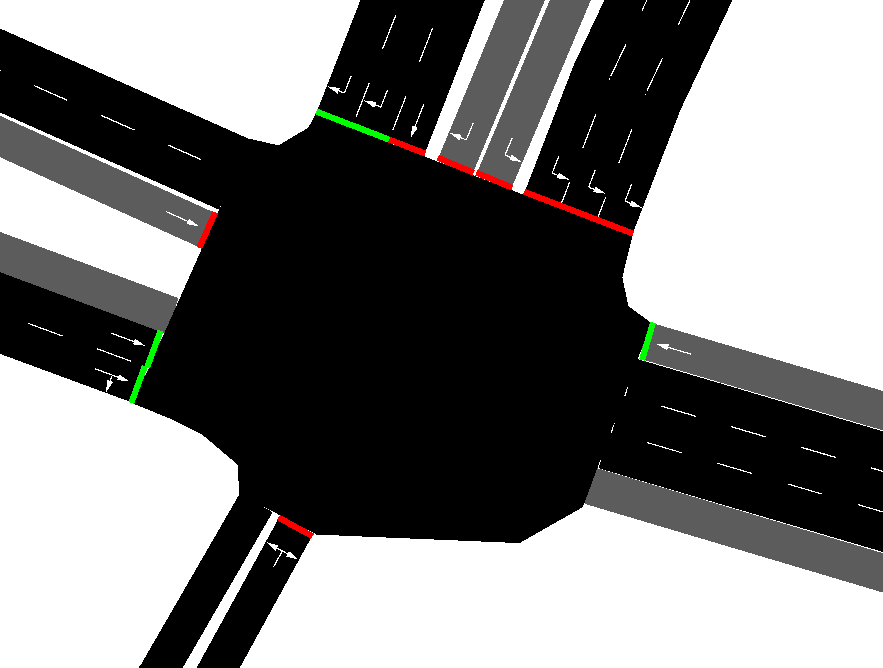
\includegraphics[width=\linewidth]{images/methodology/tl-1-street.png}
        \caption{Intersection Overview}
    \end{subfigure}
    \hfill
    \begin{subfigure}{0.45\textwidth}
        \centering
        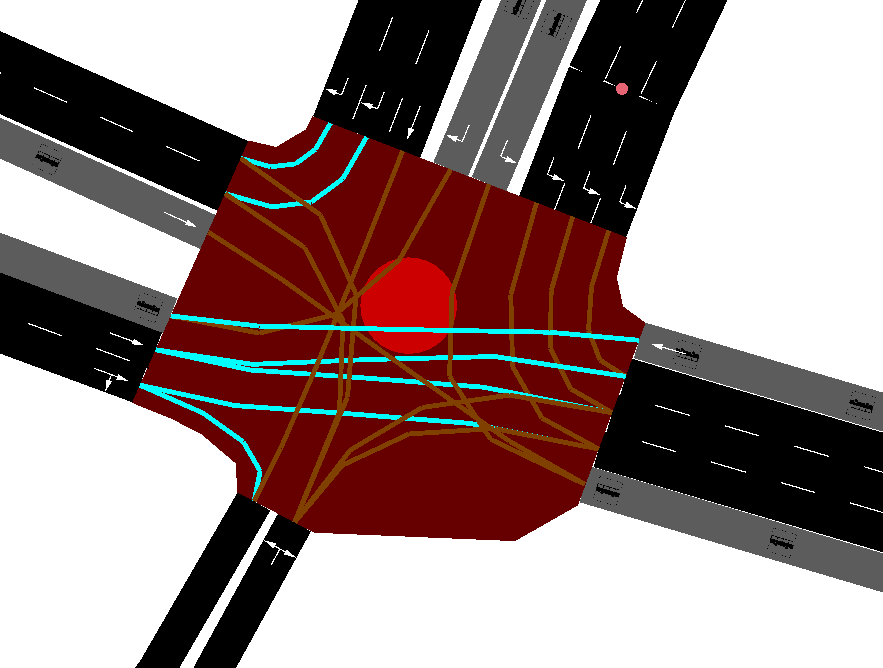
\includegraphics[width=\linewidth]{images/methodology/tl-1-directions.png}
        \caption{Lane Directions}
    \end{subfigure}
    \caption{Traffic Light 1 (TL-1)}
    \label{fig:tl-1}
\end{figure}

In Figure \ref{fig:tl-1}, we are presented with a comprehensive view of the complexity of this particular intersection. It's worth noting that this intersection stands out as one of the most challenging along Vake Street, primarily due to the intricate array of lane directions and the presence of bus lines.

\subsubsection{Intersection Complexity}
The intersection depicted in Figure \ref{fig:tl-1} exhibits a high level of complexity, characterized by the convergence of multiple road lanes and bus lines. Notably, this intersection comprises a myriad of lane directions, making it a focal point of traffic management concern.

\subsubsection{Traffic Light Phases}
Due to the inherent complexity of this intersection, Traffic Light 1 operates with a larger number of traffic light phases compared to other traffic lights along Vake Street. The additional phases are necessary to accommodate the diverse traffic movements, including the merging of bus lines and road lanes with non-standard directions.

\subsubsection{Bus Lane Configuration}
Adding to the intricacy of this intersection is the configuration of bus lanes. These bus lanes run in a reverse direction compared to the adjacent vehicle lanes. Specifically, while the vehicle lanes may be oriented from east to west, the bus lanes run from west to east. As a result, within a total of six lanes, the top two lanes serve as vehicle lanes heading east, followed by one westbound bus lane, another eastbound bus lane, and finally, two more vehicle lanes heading west. This configuration adds an extra layer of complexity to both the road layout and the corresponding traffic light control.

In summary, Traffic Light 1 at this intricate intersection serves as a prime example of the challenges presented by the unique traffic dynamics of Vake Street. The presence of bus lanes, unconventional lane directions, and a multitude of phases underscores the significance of a thorough and nuanced analysis of traffic light management in our optimization efforts.

\subsection{Traffic Light 2} \label{sec:tl-2}
Let's continue our exploration of traffic lights with an examination of Traffic Light 2, as illustrated below:

\begin{figure}[h]
    \centering
    \begin{subfigure}{0.45\textwidth}
        \centering
        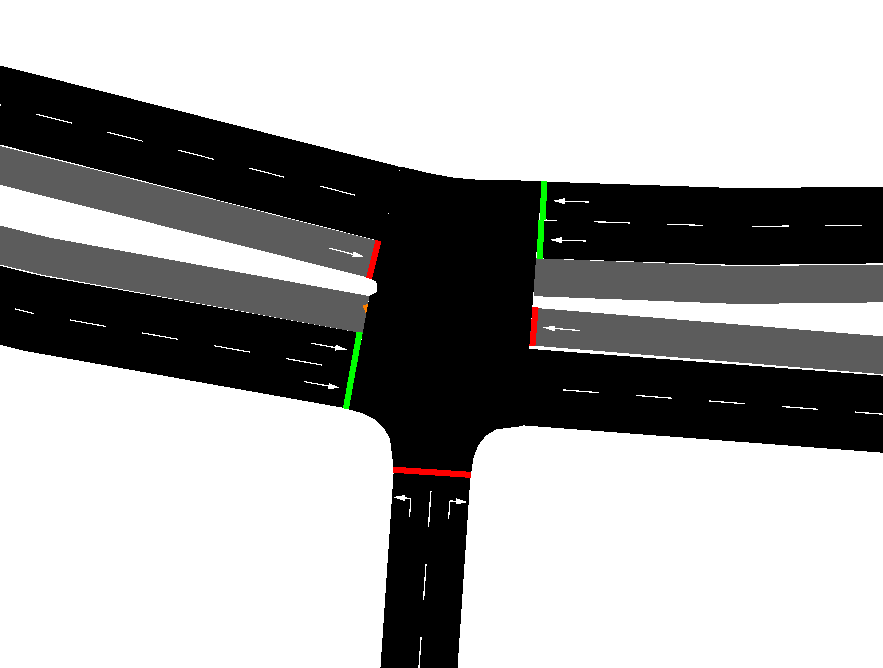
\includegraphics[width=\linewidth]{images/methodology/tl-2-street.png}
        \caption{Intersection Overview}
    \end{subfigure}
    \hfill
    \begin{subfigure}{0.45\textwidth}
        \centering
        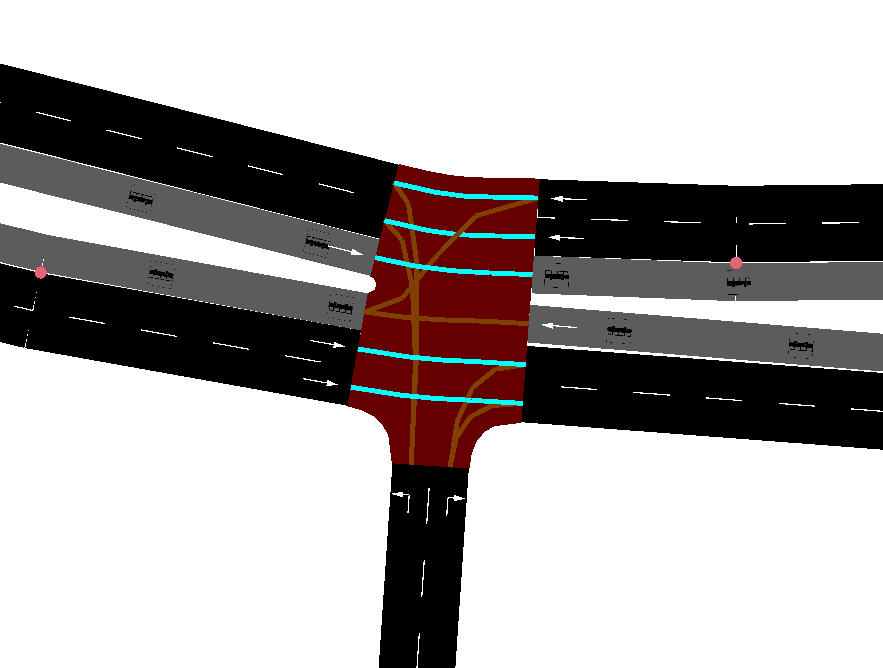
\includegraphics[width=\linewidth]{images/methodology/tl-2-directions.png}
        \caption{Lane Directions}
    \end{subfigure}
    \caption{Traffic Light 2 (TL-2)}
    \label{fig:tl-2}
\end{figure}

Comparing Traffic Light 2 in Figure \ref{fig:tl-2} to Traffic Light \hyperref[sec:tl-1]{1}, we observe a relative reduction in complexity. Notably, there is an absence of lanes heading north, simplifying the lane configuration. However, the consistent configuration of bus lanes, as detailed in previous sections, remains a common feature among all traffic lights on Vake Street.

\subsection{Traffic Light 3} \label{sec:tl-3}
Our journey through the various traffic lights brings us to Traffic Light 3, portrayed below:

\begin{figure}[h]
    \centering
    \begin{subfigure}{0.45\textwidth}
        \centering
        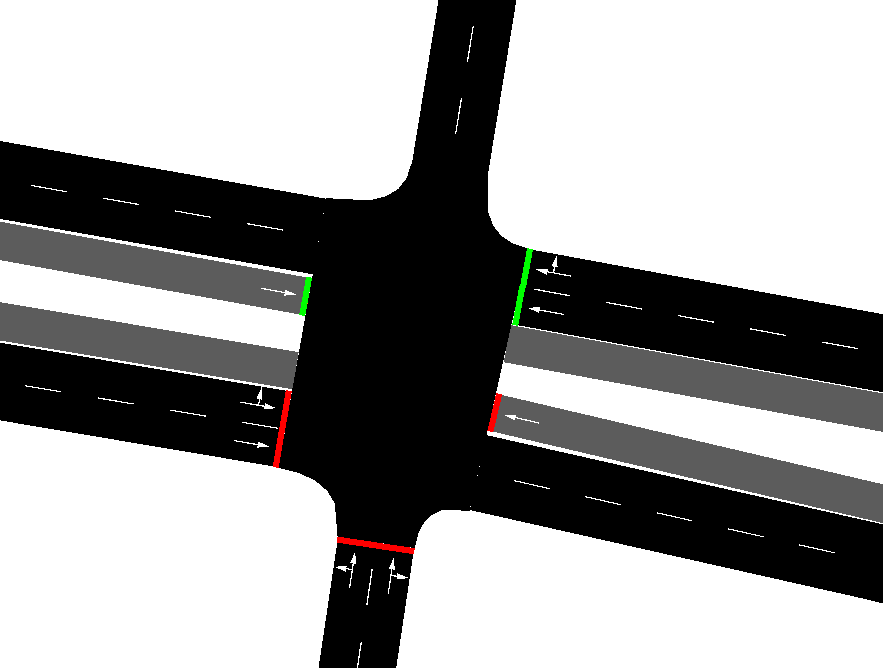
\includegraphics[width=\linewidth]{images/methodology/tl-3-street.png}
        \caption{Intersection Overview}
    \end{subfigure}
    \hfill
    \begin{subfigure}{0.45\textwidth}
        \centering
        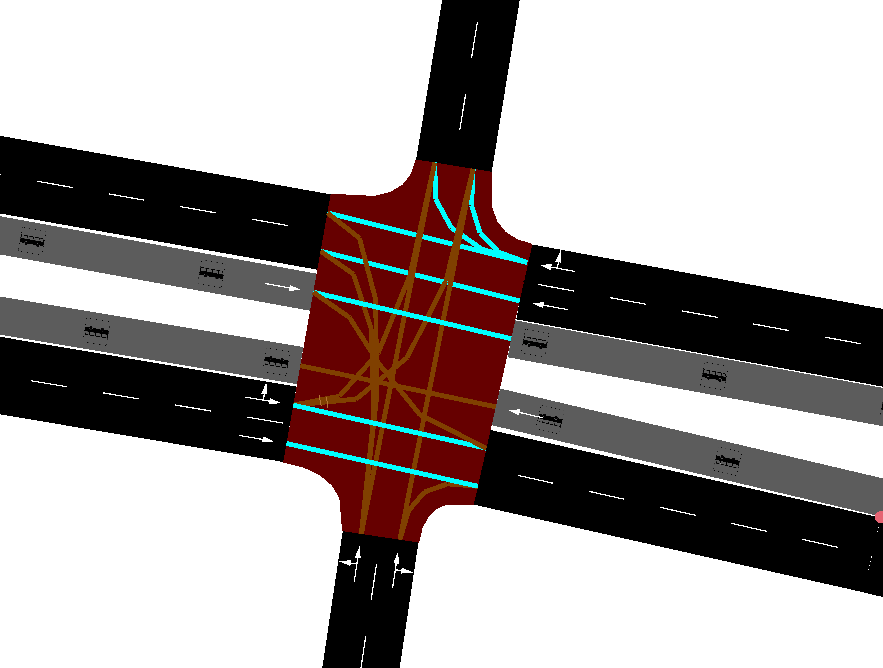
\includegraphics[width=\linewidth]{images/methodology/tl-3-directions.png}
        \caption{Lane Directions}
    \end{subfigure}
    \caption{Traffic Light 3 (TL-3)}
    \label{fig:tl-3}
\end{figure}

Traffic Light 3 introduces a heightened level of complexity compared to Traffic Light \hyperref[sec:tl-2]{2}. This complexity arises from lanes originating from the south that have the potential to traverse east and west. Additionally, it's crucial to note that southbound turns are restricted at this intersection.

\subsection{Traffic Light 4} \label{sec:tl-4}
Our exploration of traffic lights continues with Traffic Light 4, presented below:

\begin{figure}[h]
    \centering
    \begin{subfigure}{0.45\textwidth}
        \centering
        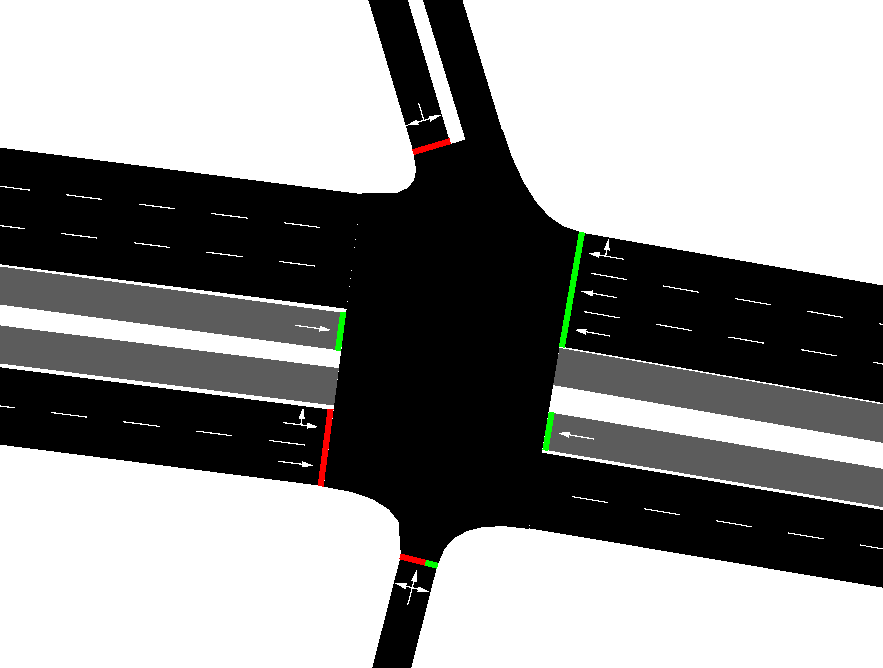
\includegraphics[width=\linewidth]{images/methodology/tl-4-street.png}
        \caption{Intersection Overview}
    \end{subfigure}
    \hfill
    \begin{subfigure}{0.45\textwidth}
        \centering
        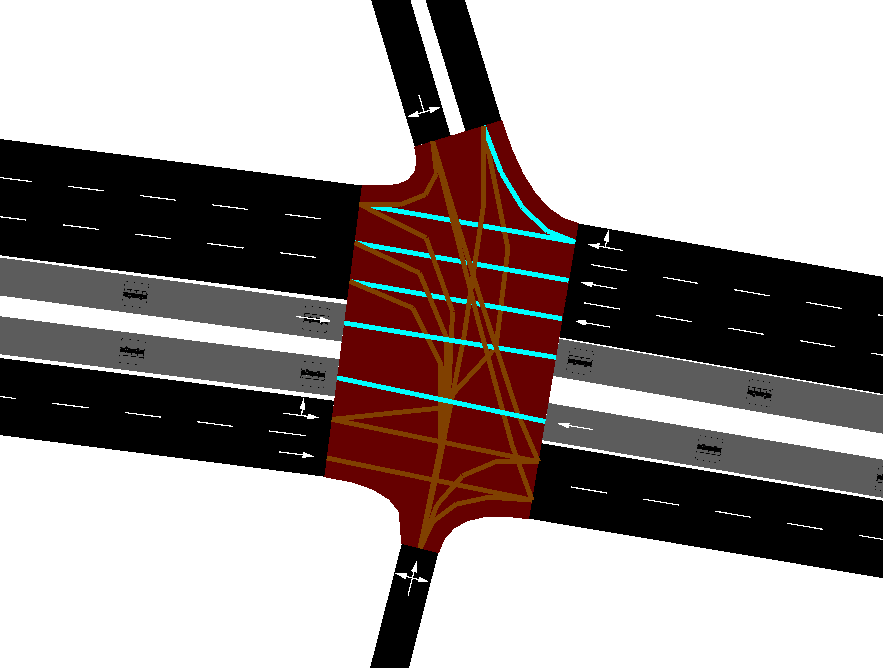
\includegraphics[width=\linewidth]{images/methodology/tl-4-directions.png}
        \caption{Lane Directions}
    \end{subfigure}
    \caption{Traffic Light 4 (TL-4)}
    \label{fig:tl-4}
\end{figure}

Traffic Light 4 presents a more complex scenario than Traffic Light \hyperref[sec:tl-3]{3}. This intersection features additional directions and a reduction in the number of lanes in certain directions. For instance, traffic from the north can now turn in both east and west directions. Furthermore, we now have three lanes dedicated to eastbound traffic, further enhancing the lane dynamics.

\subsection{Traffic Light 5} \label{sec:tl-5}
Our exploration reaches Traffic Light 5, depicted below:

\begin{figure}[h]
    \centering
    \begin{subfigure}{0.45\textwidth}
        \centering
        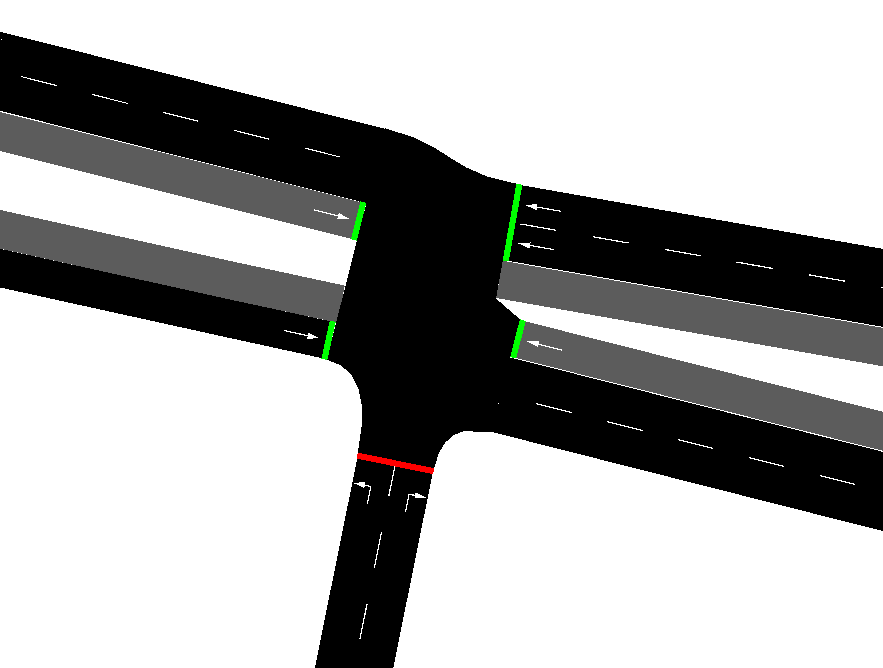
\includegraphics[width=\linewidth]{images/methodology/tl-5-street.png}
        \caption{Intersection Overview}
    \end{subfigure}
    \hfill
    \begin{subfigure}{0.45\textwidth}
        \centering
        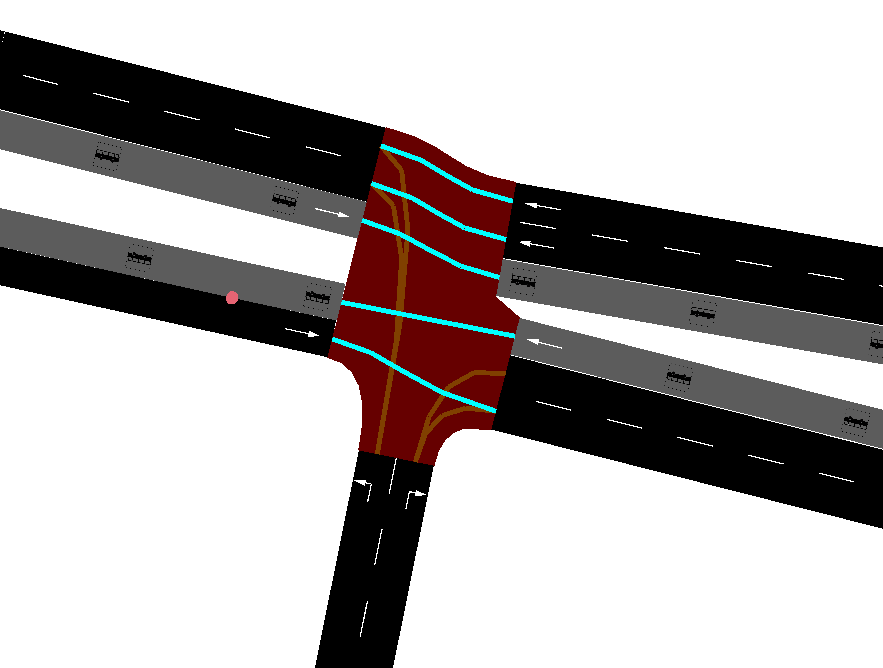
\includegraphics[width=\linewidth]{images/methodology/tl-5-directions.png}
        \caption{Lane Directions}
    \end{subfigure}
    \caption{Traffic Light 5 (TL-5)}
    \label{fig:tl-5}
\end{figure}
\newpage
As we approach the end of Vake Street, Traffic Light 5 ushers in a simpler intersection configuration. The traffic light phases here are relatively straightforward, primarily handling traffic from the south and enabling direct westbound and eastbound movements. The consistent presence of bus lanes persists in this intersection, as with the previous ones.

\subsection{Traffic Light 6} \label{sec:tl-6}
Our journey culminates with Traffic Light 6, the simplest intersection in this context, displayed below:

\begin{figure}[h]
    \centering
    \begin{subfigure}{0.45\textwidth}
        \centering
        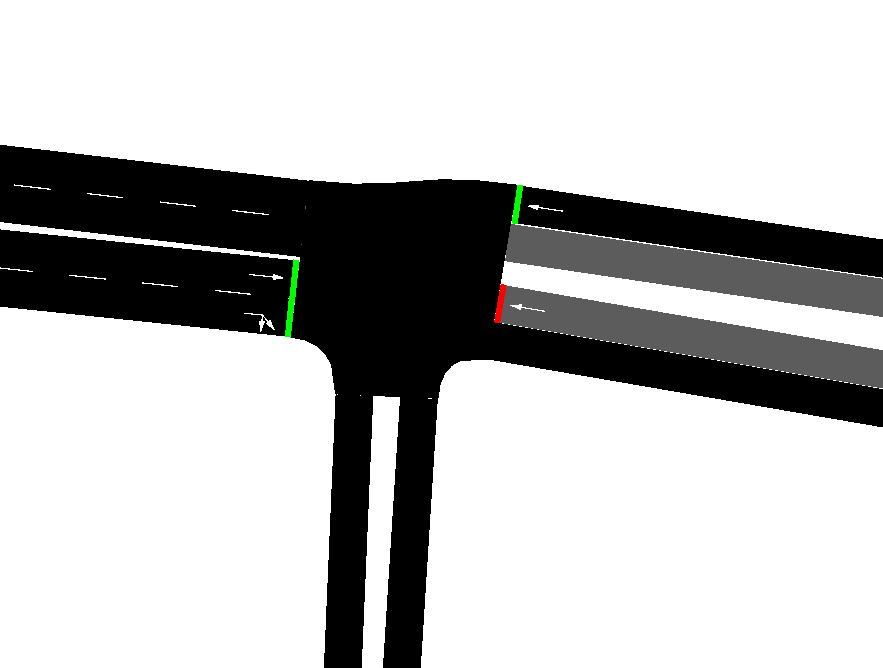
\includegraphics[width=\linewidth]{images/methodology/tl-6-street.png}
        \caption{Intersection Overview}
    \end{subfigure}
    \hfill
    \begin{subfigure}{0.45\textwidth}
        \centering
        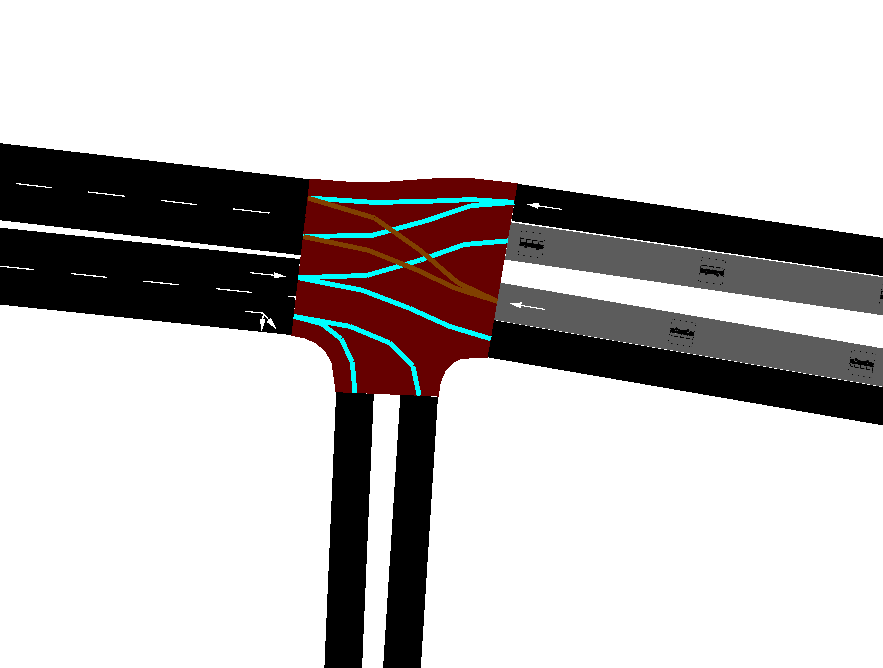
\includegraphics[width=\linewidth]{images/methodology/tl-6-directions.png}
        \caption{Lane Directions}
    \end{subfigure}
    \caption{Traffic Light 6 (TL-6)}
    \label{fig:tl-6}
\end{figure}

Traffic Light 6 represents the simplest intersection within Vake Street. Here, we primarily manage eastbound and westbound traffic, with the addition of southbound turns for westbound traffic. However, the essential role of traffic lights at this intersection is to facilitate the integration of bus lanes, which have reverse directions compared to vehicle lanes. The need for traffic lights arises from the necessity to harmonize these conflicting directions.

\subsection{Conclusion}
In the preceding sections, we have explored all six traffic lights along Vake Street. Each traffic light presents its own unique challenges, with varying levels of complexity. While some intersections are relatively straightforward, others demand nuanced control due to the intricacies of lane directions and bus lane configurations.

As we delve further into our research, we will investigate the feasibility of employing independent and multi-agent systems for traffic light control. The potential of multi-agent systems lies in their capacity to create "Green Waves," allowing for consecutive green phases tailored to specific lanes and traffic demands. This exploration aligns with our overarching goal of optimizing urban traffic flow using reinforcement learning (RL) to intelligently determine green light allocations.

\section{Traffic Simulation} \label{sec:traffic-simulation}

In this section, we delve into the realm of traffic simulation. Having outlined the construction of the Vake map in preceding sections, it is imperative to simulate the traffic conditions on this map to represent the real-world challenges accurately. To achieve this, several crucial steps were undertaken.

First and foremost, to gain an in-depth understanding of traffic flow during the busiest hours of the day, which typically span from 5:00 PM to 9:00 PM, physical visits to the Vake Street location were conducted. These on-site visits, conducted over several days with intermittent intervals, provided valuable insights into the actual traffic patterns and directions during peak hours.

Subsequently, the knowledge gleaned from these field visits was translated into a digital simulation. This was accomplished with the assistance of SUMO's $randomTrips$ tool. Despite its name, $randomTrips$ is highly versatile, allowing us to specify a wide range of options, including probability distributions, to generate traffic scenarios tailored to our needs.

The process of generating an accurate simulation, however, was not without its challenges. It required rigorous efforts and persistence. After days of meticulous work and fine-tuning, we achieved a simulation that closely mirrors the real-world traffic dynamics on Vake Street. This simulation serves as the foundation for our experiments and analysis.

For the purpose of our experiments, we opted to run the simulation for a duration of 2.5 hours, focusing specifically on the busiest period of the day. This period has been carefully selected to capture the peak traffic conditions, allowing us to conduct a series of experiments and evaluations, as detailed in the subsequent chapters.

The traffic simulation serves as a pivotal component of our research, enabling us to test and evaluate various traffic light control strategies in a controlled and representative environment. It forms the basis upon which we conduct experiments to optimize urban traffic flow using reinforcement learning-based traffic light control.


\section{Adaptation of RESCO}
In this section, we will delve into the changes made to the public RESCO repository and its adaptation for use with our specific map of Vake Street.

To enable any map to function within the RESCO framework, we must first ensure that we have a network map of SUMO and a configuration file specifying the network and simulation we intend to use. As detailed in Sections \ref{sec:map-creation}, \ref{sec:tl}, and \ref{sec:traffic-simulation}, we have already prepared these requisite files.

\subsection{Map Config}
Once we have the necessary components in place, they must be integrated into the $map\_config$ of RESCO, which takes on the following format, as illustrated in Figure \ref{fig:map-config-vake}:

\begin{figure}[h]
    \centering
    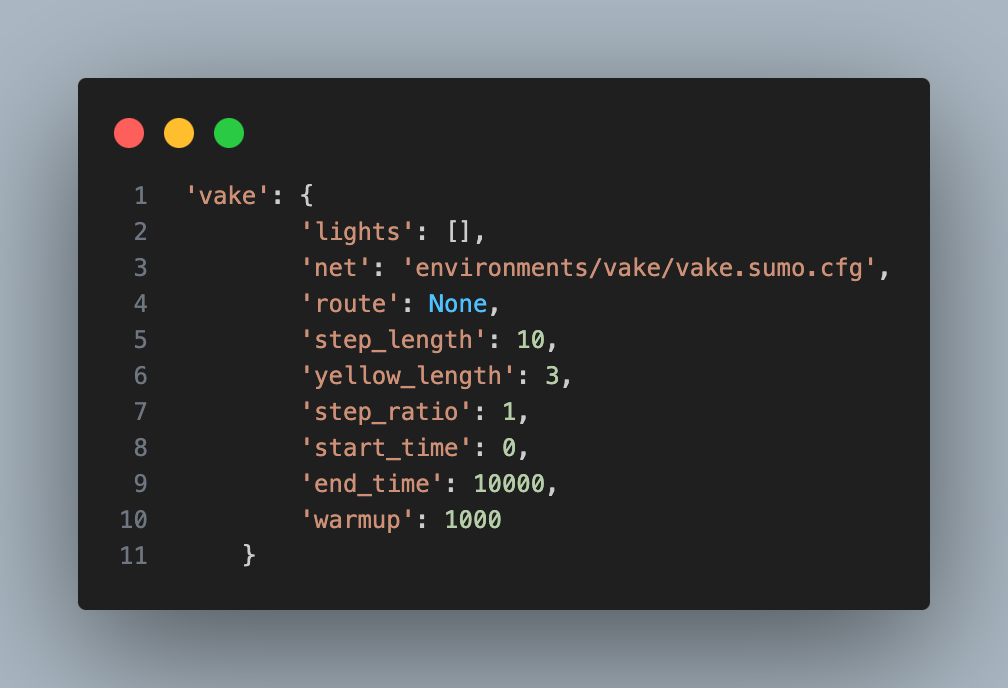
\includegraphics[width=0.8\linewidth]{images/methodology/map-config-vake.png}
    \caption{Map Config of Vake}
    \label{fig:map-config-vake}
\end{figure}

Within the $map\_config$, we specify crucial parameters, such as the fixed duration of the yellow phase, which remains constant and is not included in training due to its fixed time nature. Additionally, we define the warm-up period, indicating the number of seconds before the simulation begins to actively manage traffic signals.

\subsection{Signal Config}
Following the completion of the Map Config, we turn our attention to the Signal Config, one of the most critical configurations within the RESCO repository. Given the complexity of this configuration for multiple traffic lights, we will focus on the code snippet as shown below:

\begin{figure}[h]
    \centering
    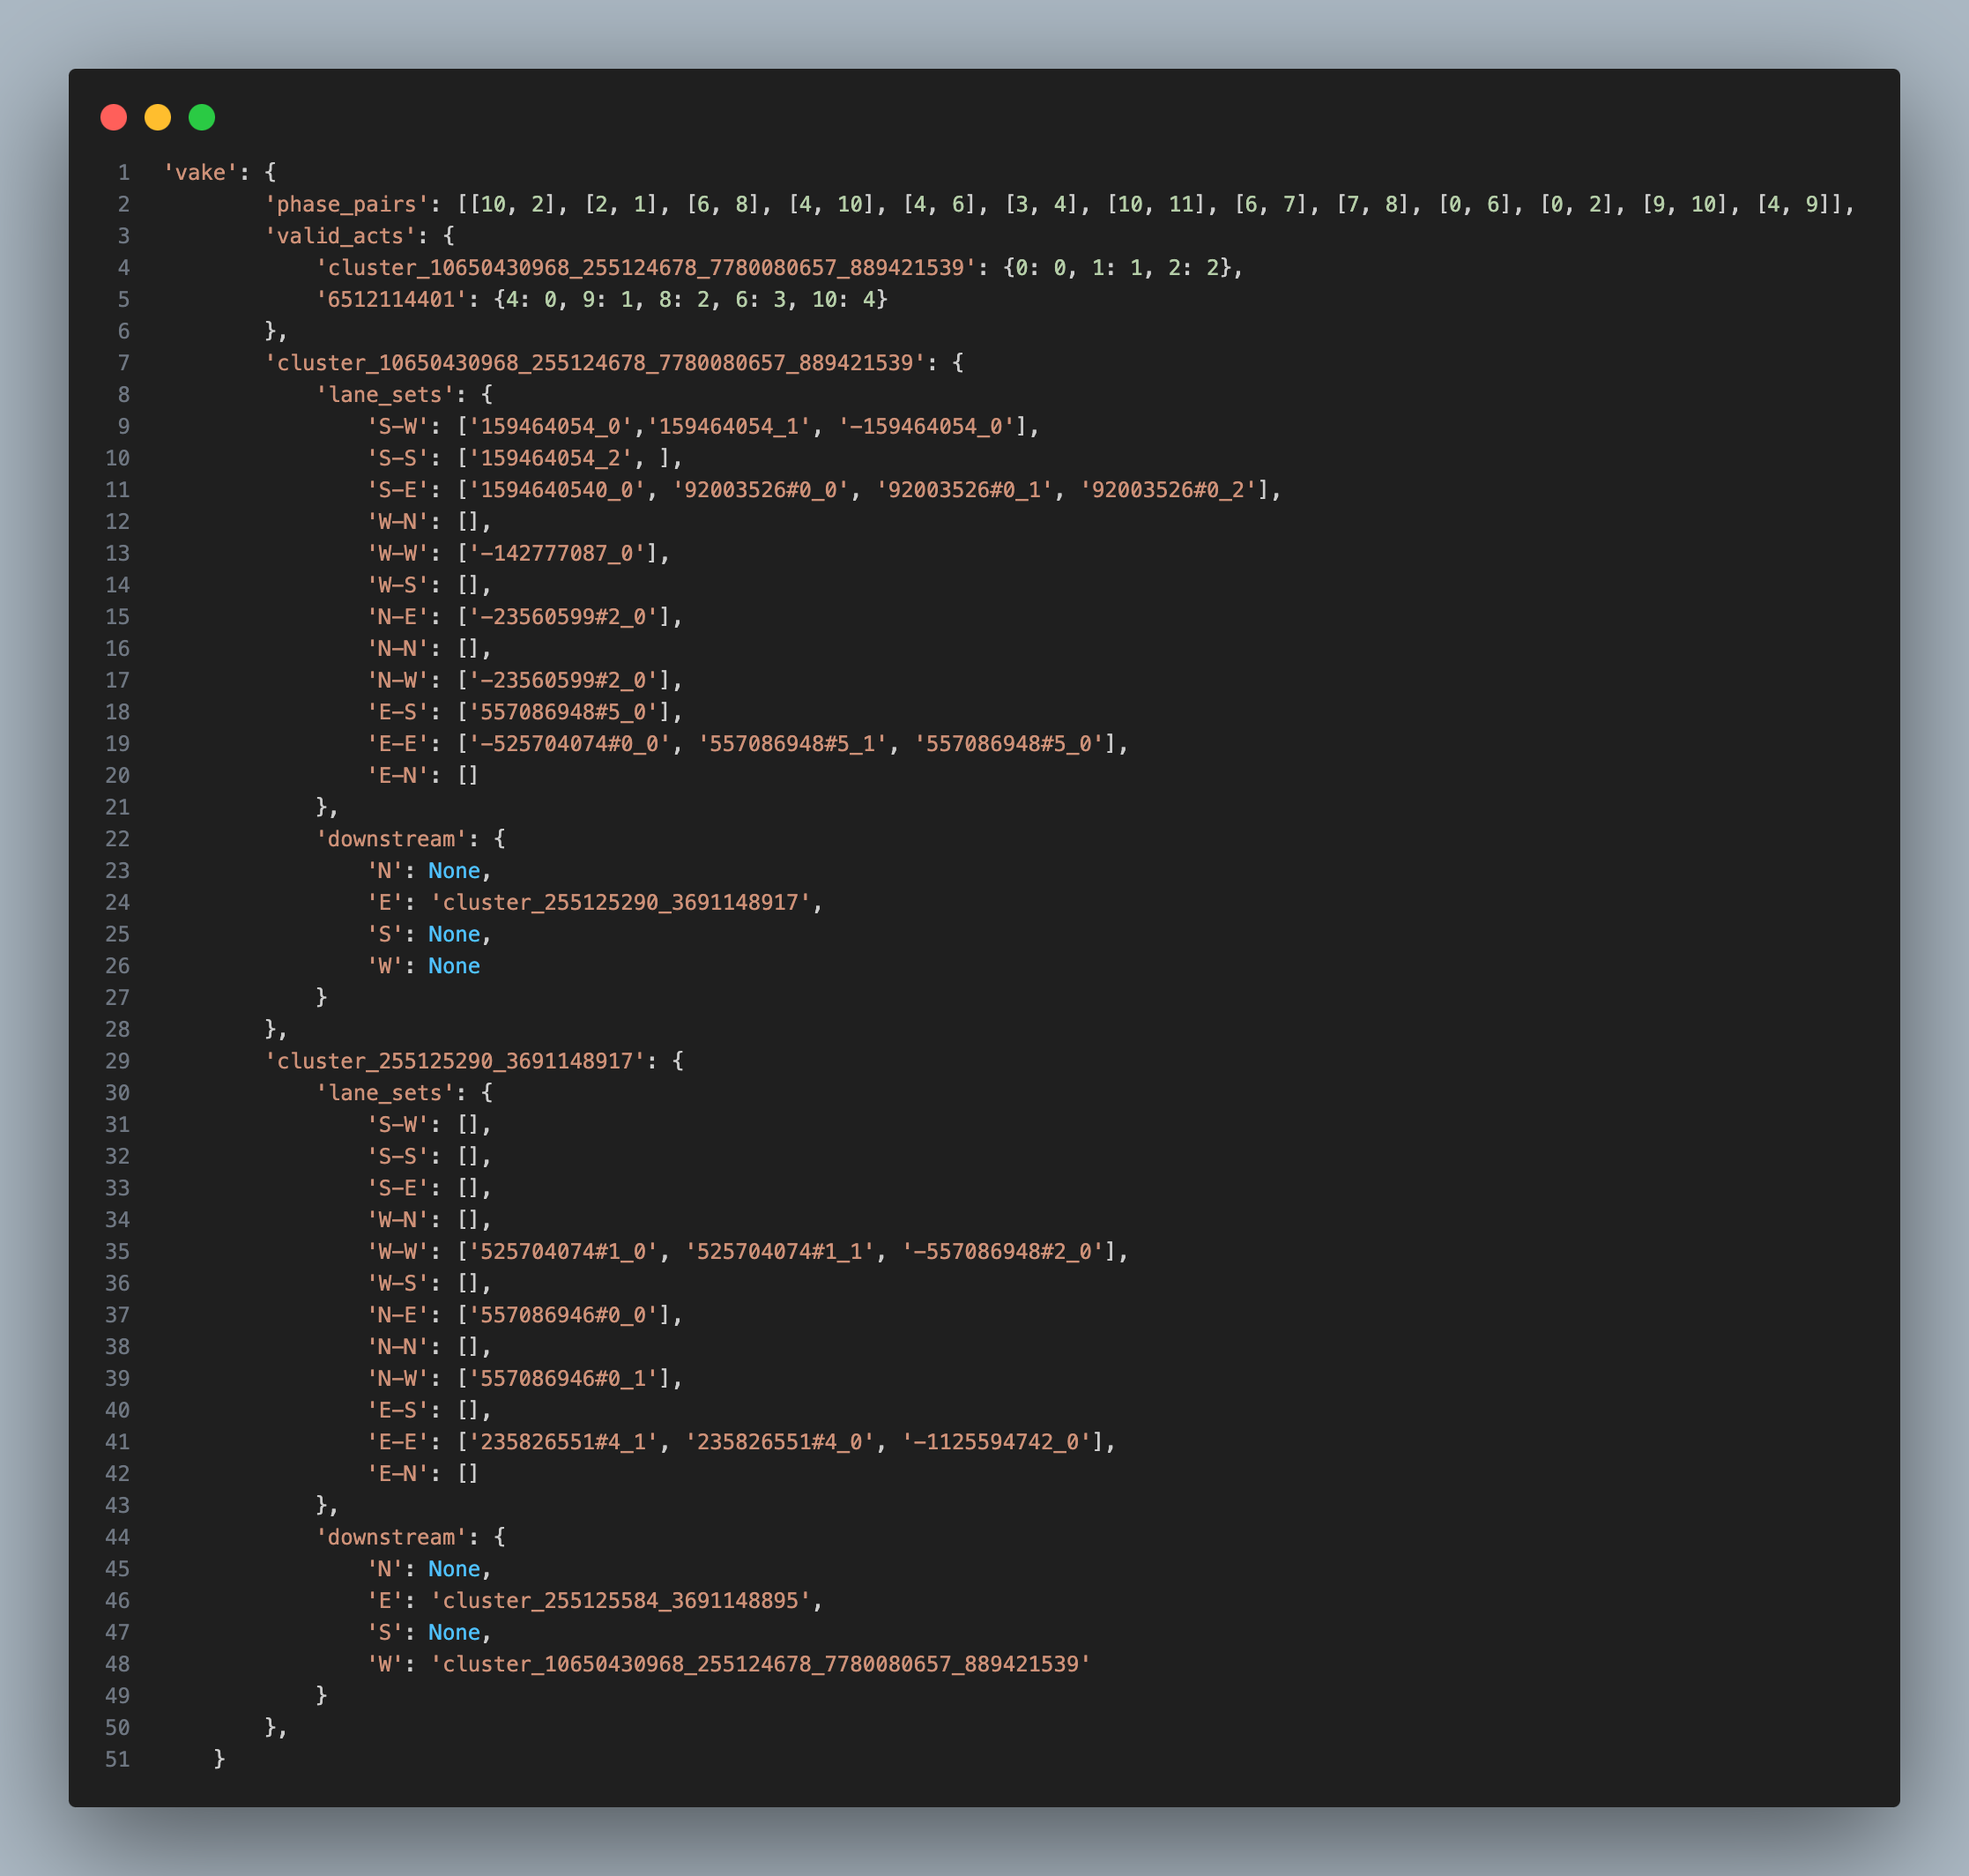
\includegraphics[width=1\linewidth]{images/methodology/signal-config-vake.png}
    \caption{Signal Config of Vake}
    \label{fig:signal-config-vake}
\end{figure}

The Signal Config, as depicted in Figure \ref{fig:signal-config-vake}, is structured as a Python dictionary, closely resembling the JSON format. This configuration encompasses various fields, including $phase\_pairs$ and $valid\_acts$. While not all agents utilize these fields, they are essential for specifying phase pairs and valid acts, dictating which phase pairs are applicable for each traffic light and phase. The indexes in phase pairs correspond to the index mapping found in Figure \ref{fig:index-trafficbound-mapping}. Each phase pair represents a combination of traffic flow directions, and their indexing defines which pairs of traffic flows can be enabled together.

\begin{figure}[h]
    \centering
    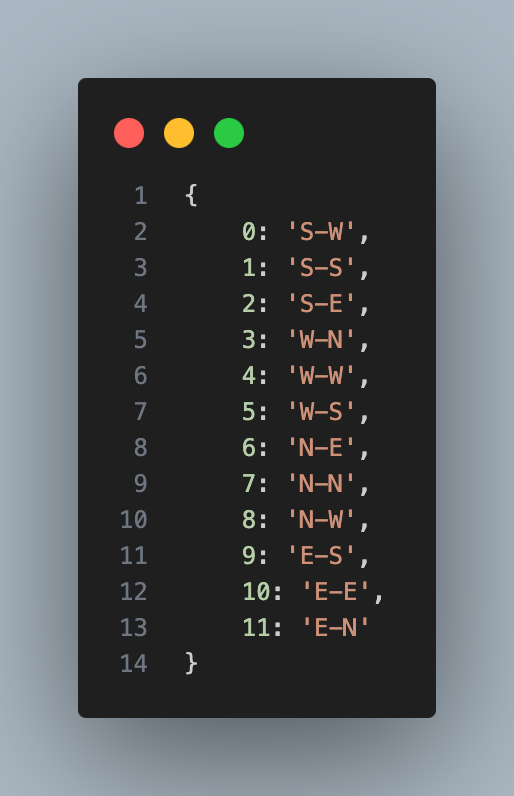
\includegraphics[width=0.3\linewidth]{images/methodology/index-trafficbound-mapping.png}
    \caption{Indexes of Traffic Flows}
    \label{fig:index-trafficbound-mapping}
\end{figure}

The Signal Config further includes fields for each traffic light, represented by their IDs in SUMO. These fields encompass $lane\_sets$ and $downstream$. In the $lane\_sets$ section, we list the IDs of individual lanes in the SUMO simulation and specify the traffic flows associated with each lane. Multiple traffic flows can be managed by a single lane, allowing for flexibility in modeling traffic patterns. The $downstream$ section identifies adjacent traffic lights, which is crucial for multi-agent coordination. For instance, if Traffic Light 1 (TL-1) has Traffic Light 2 (TL-2) as its downstream neighbor in the eastward direction, TL-2 reciprocally recognizes TL-1 as its downstream neighbor to the west.

The configuration of the Signal Config posed significant challenges, mainly due to the lack of comprehensive documentation and explanations regarding its setup. Despite opening issues in the RESCO repository, obtaining guidance proved elusive, necessitating thorough investigation and experimentation to comprehend the intricacies of the configurations.

\subsection{MDP Config}
Additionally, RESCO employs an MDP Config, which is primarily utilized by the FMA2C agent for Multi-Agent Traffic Control. The MDP Config structure includes various fields, many of which pertain to hyperparameters. However, two noteworthy fields are $management$ and $management\_neighbours$.

\subsubsection{Management}
Within the $management$ field, traffic lights are categorized into groups, with each agent assuming responsibility for a specific group. In our case, we have two agents, $top\_mgr$ and $bot\_mgr$, each overseeing three traffic lights. These agents interact with one another as part of the Multi-Agent Control framework.

\subsubsection{Management Neighbors}
The $management\_neighbours$ field specifies neighbors for each agent. While it appears relatively straightforward in our case due to the presence of just two agents, this configuration can accommodate more complex agent interactions and dependencies.

\subsection{Contribution to RESCO}
Throughout the course of this project, numerous challenges were encountered when working with RESCO, including issues with documentation and code errors. Some discrepancies in documentation and code had to be rectified to ensure successful execution. Consequently, efforts were made to address these issues, and in the spirit of open-source collaboration, a public Pull Request will be submitted to integrate the changes made to RESCO. This contribution aims to enhance the usability of RESCO for future researchers and students, mitigating some of the challenges encountered during this project.

